% Options for packages loaded elsewhere
\PassOptionsToPackage{unicode}{hyperref}
\PassOptionsToPackage{hyphens}{url}
%
\documentclass[
]{article}
\usepackage{lmodern}
\usepackage{amsmath}
\usepackage{ifxetex,ifluatex}
\ifnum 0\ifxetex 1\fi\ifluatex 1\fi=0 % if pdftex
  \usepackage[T1]{fontenc}
  \usepackage[utf8]{inputenc}
  \usepackage{textcomp} % provide euro and other symbols
  \usepackage{amssymb}
\else % if luatex or xetex
  \usepackage{unicode-math}
  \defaultfontfeatures{Scale=MatchLowercase}
  \defaultfontfeatures[\rmfamily]{Ligatures=TeX,Scale=1}
\fi
% Use upquote if available, for straight quotes in verbatim environments
\IfFileExists{upquote.sty}{\usepackage{upquote}}{}
\IfFileExists{microtype.sty}{% use microtype if available
  \usepackage[]{microtype}
  \UseMicrotypeSet[protrusion]{basicmath} % disable protrusion for tt fonts
}{}
\makeatletter
\@ifundefined{KOMAClassName}{% if non-KOMA class
  \IfFileExists{parskip.sty}{%
    \usepackage{parskip}
  }{% else
    \setlength{\parindent}{0pt}
    \setlength{\parskip}{6pt plus 2pt minus 1pt}}
}{% if KOMA class
  \KOMAoptions{parskip=half}}
\makeatother
\usepackage{xcolor}
\IfFileExists{xurl.sty}{\usepackage{xurl}}{} % add URL line breaks if available
\IfFileExists{bookmark.sty}{\usepackage{bookmark}}{\usepackage{hyperref}}
\hypersetup{
  pdftitle={Cabify - Data Science Challenge},
  pdfauthor={Luis Carrasco Tornero},
  hidelinks,
  pdfcreator={LaTeX via pandoc}}
\urlstyle{same} % disable monospaced font for URLs
\usepackage[margin=1in]{geometry}
\usepackage{color}
\usepackage{fancyvrb}
\newcommand{\VerbBar}{|}
\newcommand{\VERB}{\Verb[commandchars=\\\{\}]}
\DefineVerbatimEnvironment{Highlighting}{Verbatim}{commandchars=\\\{\}}
% Add ',fontsize=\small' for more characters per line
\usepackage{framed}
\definecolor{shadecolor}{RGB}{248,248,248}
\newenvironment{Shaded}{\begin{snugshade}}{\end{snugshade}}
\newcommand{\AlertTok}[1]{\textcolor[rgb]{0.94,0.16,0.16}{#1}}
\newcommand{\AnnotationTok}[1]{\textcolor[rgb]{0.56,0.35,0.01}{\textbf{\textit{#1}}}}
\newcommand{\AttributeTok}[1]{\textcolor[rgb]{0.77,0.63,0.00}{#1}}
\newcommand{\BaseNTok}[1]{\textcolor[rgb]{0.00,0.00,0.81}{#1}}
\newcommand{\BuiltInTok}[1]{#1}
\newcommand{\CharTok}[1]{\textcolor[rgb]{0.31,0.60,0.02}{#1}}
\newcommand{\CommentTok}[1]{\textcolor[rgb]{0.56,0.35,0.01}{\textit{#1}}}
\newcommand{\CommentVarTok}[1]{\textcolor[rgb]{0.56,0.35,0.01}{\textbf{\textit{#1}}}}
\newcommand{\ConstantTok}[1]{\textcolor[rgb]{0.00,0.00,0.00}{#1}}
\newcommand{\ControlFlowTok}[1]{\textcolor[rgb]{0.13,0.29,0.53}{\textbf{#1}}}
\newcommand{\DataTypeTok}[1]{\textcolor[rgb]{0.13,0.29,0.53}{#1}}
\newcommand{\DecValTok}[1]{\textcolor[rgb]{0.00,0.00,0.81}{#1}}
\newcommand{\DocumentationTok}[1]{\textcolor[rgb]{0.56,0.35,0.01}{\textbf{\textit{#1}}}}
\newcommand{\ErrorTok}[1]{\textcolor[rgb]{0.64,0.00,0.00}{\textbf{#1}}}
\newcommand{\ExtensionTok}[1]{#1}
\newcommand{\FloatTok}[1]{\textcolor[rgb]{0.00,0.00,0.81}{#1}}
\newcommand{\FunctionTok}[1]{\textcolor[rgb]{0.00,0.00,0.00}{#1}}
\newcommand{\ImportTok}[1]{#1}
\newcommand{\InformationTok}[1]{\textcolor[rgb]{0.56,0.35,0.01}{\textbf{\textit{#1}}}}
\newcommand{\KeywordTok}[1]{\textcolor[rgb]{0.13,0.29,0.53}{\textbf{#1}}}
\newcommand{\NormalTok}[1]{#1}
\newcommand{\OperatorTok}[1]{\textcolor[rgb]{0.81,0.36,0.00}{\textbf{#1}}}
\newcommand{\OtherTok}[1]{\textcolor[rgb]{0.56,0.35,0.01}{#1}}
\newcommand{\PreprocessorTok}[1]{\textcolor[rgb]{0.56,0.35,0.01}{\textit{#1}}}
\newcommand{\RegionMarkerTok}[1]{#1}
\newcommand{\SpecialCharTok}[1]{\textcolor[rgb]{0.00,0.00,0.00}{#1}}
\newcommand{\SpecialStringTok}[1]{\textcolor[rgb]{0.31,0.60,0.02}{#1}}
\newcommand{\StringTok}[1]{\textcolor[rgb]{0.31,0.60,0.02}{#1}}
\newcommand{\VariableTok}[1]{\textcolor[rgb]{0.00,0.00,0.00}{#1}}
\newcommand{\VerbatimStringTok}[1]{\textcolor[rgb]{0.31,0.60,0.02}{#1}}
\newcommand{\WarningTok}[1]{\textcolor[rgb]{0.56,0.35,0.01}{\textbf{\textit{#1}}}}
\usepackage{graphicx}
\makeatletter
\def\maxwidth{\ifdim\Gin@nat@width>\linewidth\linewidth\else\Gin@nat@width\fi}
\def\maxheight{\ifdim\Gin@nat@height>\textheight\textheight\else\Gin@nat@height\fi}
\makeatother
% Scale images if necessary, so that they will not overflow the page
% margins by default, and it is still possible to overwrite the defaults
% using explicit options in \includegraphics[width, height, ...]{}
\setkeys{Gin}{width=\maxwidth,height=\maxheight,keepaspectratio}
% Set default figure placement to htbp
\makeatletter
\def\fps@figure{htbp}
\makeatother
\setlength{\emergencystretch}{3em} % prevent overfull lines
\providecommand{\tightlist}{%
  \setlength{\itemsep}{0pt}\setlength{\parskip}{0pt}}
\setcounter{secnumdepth}{-\maxdimen} % remove section numbering
\ifluatex
  \usepackage{selnolig}  % disable illegal ligatures
\fi

\title{Cabify - Data Science Challenge}
\author{Luis Carrasco Tornero}
\date{June 3, 2018}

\begin{document}
\maketitle

\hypertarget{part-1-experiment-design}{%
\subsection{Part 1: Experiment design}\label{part-1-experiment-design}}

\textbf{AirBnB Professional photography: 1. Provide full details about
how you will run experiments to assess the impact of this service on
both hosts and guests. How will you ensure that the experiments are
valid and not biased?}

Two different approaches could be used to test whether professional
photography services are impacting the success of the properties.

\begin{enumerate}
\def\labelenumi{\arabic{enumi})}
\item
  Experiment based on the comparison between properties using the
  services against those not using the service.
\item
  Temporal comparison, analyzing the success increase (or not) of
  properties that adopted the professional photography but did not used
  it in the past.
\end{enumerate}

For \textbf{experiment 1)}, data of both hosts and guests will be
compiled. Examples of the data compiled would be:

\begin{itemize}
\item
  Host data: Number of visits, number of bookings, price/night/guest,
  city, location, property characteristics (number of bedrooms, bed
  size, etc.).
\item
  Guest data: Number of visits, type of booked host, time of each visit,
  rating of host description `accuracy'.
\end{itemize}

The ratio visits/booking would be compared between hosts with and
without photography service. Time of each visit for guests of hosts with
and without the service would be compared. Also the ratio of bookings
for hosts with and without service will be compared for similar type
hosts (see avoiding biases section). Comparison of the `accuracy' rating
would be done. Stats: The analysis could be performed using tests for
equality of means.

\textbf{Experiment 2)} would analyze success changes of properties
changing from not using service to using one (and the opposite
direction, if there are cases). This experiment would analyze hosts
(using the data of experiment 1). The price of the property, the number
of bookings per unit of time, as well as the ratio visits/bookings will
be compared from before and after using the service. Increases in the
price after adopting the service would be especially useful. Stats: Step
functions (in comparison with continuous functions) and time-series
analysis based (i.e.~change-point detection) methods could be used.

\textbf{Avoiding biases:} Comparison between photography service users
and not users is not trivial because the booking success is affected by
many variables, such as the price or quality of the property. In order
to avoid those biases, separate analysis controlling for those variables
are needed. This are a few examples of how to avoid this biases:

\begin{itemize}
\item
  Use data only from 2015. The launch of identity verification, double
  blind reviews, increase of PR for AirBnB and the high quality of smart
  phones cameras could by decreasing the relative importance of the
  professional photography. Using data from before 2015 could give an
  overestimated value of the service.
\item
  Compare data for same price ranges: More expensive hosts could be more
  dependent on high quality photography, as people staying at pricey
  properties might be looking for beauty. Guests looking for cheaper
  properties might not be looking for pretty-looking properties but for
  convenient ones.
\item
  Compare data for similar locations: Very busy locations could be less
  influenced by the quality of the photography, as visitors look for
  cheaper deals no matter of the looks of the property. On the other
  hand, countryside locations could be relying on the looks.
\item
  Comparing by price and location might not be enough to avoid quality
  bias, as some properties might have better facilities. Number of
  rooms, bathrooms, room size or facilities could be compared. Some
  index could be built to compile all this characteristics into a
  `quality' measure. The analysis should compare properties with similar
  quality.
\end{itemize}

Considering all these biases would be fundamental, as the results could
show that the best strategy might be to offer the service just to
expensive properties (the service is more important and the benefit for
AirBnB is bigger), or to properties located in the countryside.

\hypertarget{part-2-result-analysis}{%
\subsection{Part 2: Result analysis}\label{part-2-result-analysis}}

\emph{Pick-up time optimization challenge}

In order to the answer the questions proposed in the challenge: ``should
the company move towards \emph{road} distance?'', the main purpose of
the data analysis is to clarify whether or not the duration of the rides
to pick up the customers are shorter for the \emph{road} vehicles than
for the \emph{linear} vehicles.

To do that, the focus will be on the \emph{going\_to\_pickup} data, and
the mean values for the duration of the trips will be analysed for
different parameters.

First, the data is extracted:

\begin{Shaded}
\begin{Highlighting}[]
\NormalTok{json\_file }\OtherTok{\textless{}{-}} \StringTok{"intervals\_challenge.json"}
\NormalTok{data }\OtherTok{\textless{}{-}} \FunctionTok{fromJSON}\NormalTok{(}\FunctionTok{sprintf}\NormalTok{(}\StringTok{"[\%s]"}\NormalTok{,}\FunctionTok{paste}\NormalTok{(}\FunctionTok{readLines}\NormalTok{(json\_file),}\AttributeTok{collapse =} \StringTok{","}\NormalTok{)))}
\NormalTok{df\_raw }\OtherTok{\textless{}{-}} \FunctionTok{do.call}\NormalTok{(rbind.data.frame,data)}
\FunctionTok{print}\NormalTok{(}\FunctionTok{paste}\NormalTok{(}\StringTok{"Number of data elements = "}\NormalTok{,}\FunctionTok{nrow}\NormalTok{(df\_raw)}\SpecialCharTok{*}\FunctionTok{ncol}\NormalTok{(df\_raw),}\AttributeTok{sep=}\StringTok{""}\NormalTok{))}
\end{Highlighting}
\end{Shaded}

\begin{verbatim}
## [1] "Number of data elements = 1156190"
\end{verbatim}

The data contains more than a million elements. The size of the data
could represent slow computing times so some data cleansing is needed.
The purpose of the challenge is to evaluate whether the new \emph{road}
assignment will reduce the pick up duration, so the other intervals data
are not needed. Other variables, such as distance or vehicles ids are
not needed for our analysis either.

\begin{Shaded}
\begin{Highlighting}[]
\CommentTok{\# Subset to "going\_to\_pickup"}
\NormalTok{df\_sub1 }\OtherTok{\textless{}{-}} \FunctionTok{subset}\NormalTok{(df\_raw,type}\SpecialCharTok{==}\StringTok{"going\_to\_pickup"}\NormalTok{)}
\CommentTok{\# Exclude non{-}used variables}
\NormalTok{vars }\OtherTok{\textless{}{-}} \FunctionTok{names}\NormalTok{(df\_sub1) }\SpecialCharTok{\%in\%} \FunctionTok{c}\NormalTok{(}\StringTok{"distance"}\NormalTok{, }\StringTok{"vehicle\_id"}\NormalTok{, }\StringTok{"type"}\NormalTok{)}
\NormalTok{df\_sub }\OtherTok{\textless{}{-}}\NormalTok{ df\_sub1[}\SpecialCharTok{!}\NormalTok{vars]}
\CommentTok{\# Remove non{-}desired data}
\FunctionTok{rm}\NormalTok{(data,df\_raw,df\_sub1)}

\FunctionTok{print}\NormalTok{(}\FunctionTok{paste}\NormalTok{(}\StringTok{"Number of data elements = "}\NormalTok{,}\FunctionTok{nrow}\NormalTok{(df\_sub)}\SpecialCharTok{*}\FunctionTok{ncol}\NormalTok{(df\_sub),}\AttributeTok{sep=}\StringTok{""}\NormalTok{))}
\end{Highlighting}
\end{Shaded}

\begin{verbatim}
## [1] "Number of data elements = 234040"
\end{verbatim}

Now the number of elements have been reduce more than 4 times.

The \emph{trip\_id} needs to be reclassified into \emph{road} and
\emph{linear} factors in order to be analysed:

\begin{Shaded}
\begin{Highlighting}[]
\CommentTok{\# Assign to "road"}
\NormalTok{df\_sub}\SpecialCharTok{$}\NormalTok{trip\_id }\OtherTok{\textless{}{-}}  \FunctionTok{gsub}\NormalTok{(}\StringTok{"\^{}0}\SpecialCharTok{\textbackslash{}\textbackslash{}}\StringTok{w+|\^{}1}\SpecialCharTok{\textbackslash{}\textbackslash{}}\StringTok{w+|\^{}2}\SpecialCharTok{\textbackslash{}\textbackslash{}}\StringTok{w+|\^{}3}\SpecialCharTok{\textbackslash{}\textbackslash{}}\StringTok{w+|\^{}4}\SpecialCharTok{\textbackslash{}\textbackslash{}}\StringTok{w+|\^{}5}\SpecialCharTok{\textbackslash{}\textbackslash{}}\StringTok{w+|\^{}6}\SpecialCharTok{\textbackslash{}\textbackslash{}}\StringTok{w+|\^{}7}\SpecialCharTok{\textbackslash{}\textbackslash{}}\StringTok{w+|\^{}8}\SpecialCharTok{\textbackslash{}\textbackslash{}}\StringTok{w+"}\NormalTok{, }
                        \StringTok{"road"}\NormalTok{, df\_sub}\SpecialCharTok{$}\NormalTok{trip\_id)}
\CommentTok{\# Assign to "linear"}
\NormalTok{df\_sub}\SpecialCharTok{$}\NormalTok{trip\_id }\OtherTok{\textless{}{-}} \FunctionTok{gsub}\NormalTok{(}\StringTok{"\^{}9}\SpecialCharTok{\textbackslash{}\textbackslash{}}\StringTok{w+|\^{}a}\SpecialCharTok{\textbackslash{}\textbackslash{}}\StringTok{w+|\^{}b}\SpecialCharTok{\textbackslash{}\textbackslash{}}\StringTok{w+|\^{}c}\SpecialCharTok{\textbackslash{}\textbackslash{}}\StringTok{w+|\^{}d}\SpecialCharTok{\textbackslash{}\textbackslash{}}\StringTok{w+|\^{}e}\SpecialCharTok{\textbackslash{}\textbackslash{}}\StringTok{w+|\^{}f}\SpecialCharTok{\textbackslash{}\textbackslash{}}\StringTok{w+"}\NormalTok{, }
                        \StringTok{"linear"}\NormalTok{, df\_sub}\SpecialCharTok{$}\NormalTok{trip\_id)}
\end{Highlighting}
\end{Shaded}

Now we want to see how the data looks like without controlling for city,
time of the day, or ride duration range. To do that, boxplots for each
assignment (\emph{road} and \emph{linear}) showing the median and
quartiles are used:

\begin{Shaded}
\begin{Highlighting}[]
\NormalTok{p1 }\OtherTok{\textless{}{-}} \FunctionTok{ggplot}\NormalTok{(}\FunctionTok{aes}\NormalTok{(}\AttributeTok{y =} \FunctionTok{as.numeric}\NormalTok{(duration), }\AttributeTok{x =} \FunctionTok{as.factor}\NormalTok{(trip\_id)), }
             \AttributeTok{data =}\NormalTok{ df\_sub) }\SpecialCharTok{+} \FunctionTok{geom\_boxplot}\NormalTok{()}
\NormalTok{p1 }\SpecialCharTok{+} \FunctionTok{xlab}\NormalTok{(}\StringTok{"Assigment"}\NormalTok{) }\SpecialCharTok{+} \FunctionTok{ylab}\NormalTok{(}\StringTok{"Duration (s)"}\NormalTok{) }
\end{Highlighting}
\end{Shaded}

\begin{verbatim}
## Warning in FUN(X[[i]], ...): NAs introduced by coercion

## Warning in FUN(X[[i]], ...): NAs introduced by coercion
\end{verbatim}

\begin{verbatim}
## Warning: Removed 299 rows containing non-finite values (stat_boxplot).
\end{verbatim}

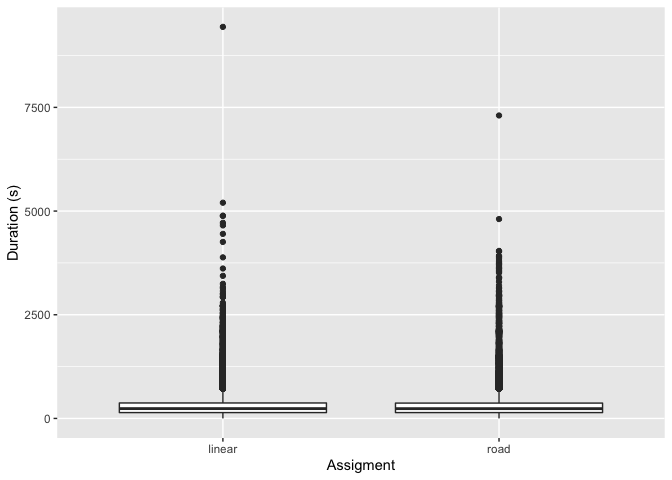
\includegraphics{cabify_challenge_files/figure-latex/unnamed-chunk-5-1.pdf}

Median values look virtually identical. But to test whether
\emph{linear} and \emph{road} assignment is providing different
duration, a statistical test is needed. To choose the proper test to be
used for our data, we need to first test whether the data is normally
distributed. A Shaphiro-Wilk normality test for \emph{duration} is used
for each assignment:

\begin{Shaded}
\begin{Highlighting}[]
\CommentTok{\# Shapiro{-}Wilk normality test for road duration}
\FunctionTok{with}\NormalTok{(df\_sub[}\FunctionTok{sample}\NormalTok{(}\DecValTok{1}\SpecialCharTok{:}\FunctionTok{nrow}\NormalTok{(df\_sub),}\DecValTok{5000}\NormalTok{),], }
     \FunctionTok{shapiro.test}\NormalTok{(}\FunctionTok{as.numeric}\NormalTok{(duration[trip\_id }\SpecialCharTok{==} \StringTok{"linear"}\NormalTok{])))}
\end{Highlighting}
\end{Shaded}

\begin{verbatim}
## Warning in stopifnot(is.numeric(x)): NAs introduced by coercion
\end{verbatim}

\begin{verbatim}
## 
##  Shapiro-Wilk normality test
## 
## data:  as.numeric(duration[trip_id == "linear"])
## W = 0.73094, p-value < 2.2e-16
\end{verbatim}

\begin{Shaded}
\begin{Highlighting}[]
\CommentTok{\# Shapiro{-}Wilk normality test for linear duration}
\FunctionTok{with}\NormalTok{(df\_sub[}\FunctionTok{sample}\NormalTok{(}\DecValTok{1}\SpecialCharTok{:}\FunctionTok{nrow}\NormalTok{(df\_sub),}\DecValTok{5000}\NormalTok{),], }
     \FunctionTok{shapiro.test}\NormalTok{(}\FunctionTok{as.numeric}\NormalTok{(duration[trip\_id }\SpecialCharTok{==} \StringTok{"road"}\NormalTok{])))}
\end{Highlighting}
\end{Shaded}

\begin{verbatim}
## Warning in stopifnot(is.numeric(x)): NAs introduced by coercion
\end{verbatim}

\begin{verbatim}
## 
##  Shapiro-Wilk normality test
## 
## data:  as.numeric(duration[trip_id == "road"])
## W = 0.67319, p-value < 2.2e-16
\end{verbatim}

The W values and p-values indicate that the data is not normally
distributed. Because of this, t-tests cannot be used. We then have to
run a Wilcoxon test for non-normal distributed data in order to test the
equality of the mean values of \emph{duration}.

\begin{Shaded}
\begin{Highlighting}[]
\FunctionTok{wilcox.test}\NormalTok{(}\FunctionTok{as.numeric}\NormalTok{(df\_sub}\SpecialCharTok{$}\NormalTok{duration[df\_sub}\SpecialCharTok{$}\NormalTok{trip\_id}\SpecialCharTok{==}\StringTok{"road"}\NormalTok{]), }
            \FunctionTok{as.numeric}\NormalTok{(df\_sub}\SpecialCharTok{$}\NormalTok{duration[df\_sub}\SpecialCharTok{$}\NormalTok{trip\_id}\SpecialCharTok{==}\StringTok{"linear"}\NormalTok{]), }
            \AttributeTok{alternative =} \StringTok{"two.sided"}\NormalTok{)}
\end{Highlighting}
\end{Shaded}

\begin{verbatim}
## Warning in wilcox.test(as.numeric(df_sub$duration[df_sub$trip_id == "road"]), :
## NAs introduced by coercion
\end{verbatim}

\begin{verbatim}
## Warning in wilcox.test.default(as.numeric(df_sub$duration[df_sub$trip_id == :
## NAs introduced by coercion
\end{verbatim}

\begin{verbatim}
## 
##  Wilcoxon rank sum test with continuity correction
## 
## data:  as.numeric(df_sub$duration[df_sub$trip_id == "road"]) and as.numeric(df_sub$duration[df_sub$trip_id == "linear"])
## W = 414584657, p-value = 0.4689
## alternative hypothesis: true location shift is not equal to 0
\end{verbatim}

The Wilcoxon test indicates that we can not assume that the means are
different. In other words, the means of \emph{duration} are not
different, and there is no effect of the assignment type on the duration
of the rides.

We can compare the mean duration values for \emph{linear} and
\emph{road}:

\begin{Shaded}
\begin{Highlighting}[]
\FunctionTok{mean}\NormalTok{(}\FunctionTok{as.numeric}\NormalTok{(df\_sub}\SpecialCharTok{$}\NormalTok{duration[df\_sub}\SpecialCharTok{$}\NormalTok{trip\_id}\SpecialCharTok{==}\StringTok{"linear"}\NormalTok{]))}
\end{Highlighting}
\end{Shaded}

\begin{verbatim}
## Warning in mean(as.numeric(df_sub$duration[df_sub$trip_id == "linear"])): NAs
## introduced by coercion
\end{verbatim}

\begin{verbatim}
## [1] NA
\end{verbatim}

\begin{Shaded}
\begin{Highlighting}[]
\FunctionTok{mean}\NormalTok{(}\FunctionTok{as.numeric}\NormalTok{(df\_sub}\SpecialCharTok{$}\NormalTok{duration[df\_sub}\SpecialCharTok{$}\NormalTok{trip\_id}\SpecialCharTok{==}\StringTok{"road"}\NormalTok{]))}
\end{Highlighting}
\end{Shaded}

\begin{verbatim}
## Warning in mean(as.numeric(df_sub$duration[df_sub$trip_id == "road"])): NAs
## introduced by coercion
\end{verbatim}

\begin{verbatim}
## [1] NA
\end{verbatim}

The \emph{road} assignment was, in average, only 2 seconds faster.
Although this is not statistically significant and this difference could
be due to randomness.

Next, the same analysis was performed for different intervals of
duration time. One could argue that the \emph{normal} assignment could
work better for larger distances (and therefore larger duration), so
that the mean value considering all durations is not taking into account
some particular duration times. Larger distances mean more uncertainty
and therefore \emph{normal} could work better.

To test this, an analysis was done for different duration intervals with
same results. Preliminary analysis showed smaller duration for the
\emph{road} assignment when the duration was large (distant places), and
no differences for small durations. For example, this is the difference
for durations above 3000 seconds:

\begin{Shaded}
\begin{Highlighting}[]
\NormalTok{p2 }\OtherTok{\textless{}{-}} \FunctionTok{ggplot}\NormalTok{(}\FunctionTok{aes}\NormalTok{(}\AttributeTok{y =} \FunctionTok{as.numeric}\NormalTok{(duration), }\AttributeTok{x =} \FunctionTok{as.factor}\NormalTok{(trip\_id)), }
             \AttributeTok{data =}\NormalTok{ df\_sub[}\FunctionTok{as.numeric}\NormalTok{(df\_sub}\SpecialCharTok{$}\NormalTok{duration)}\SpecialCharTok{\textgreater{}}\DecValTok{3000}\NormalTok{,]) }\SpecialCharTok{+} \FunctionTok{geom\_boxplot}\NormalTok{()}
\end{Highlighting}
\end{Shaded}

\begin{verbatim}
## Warning in `[.data.frame`(df_sub, as.numeric(df_sub$duration) > 3000, ): NAs
## introduced by coercion
\end{verbatim}

\begin{Shaded}
\begin{Highlighting}[]
\NormalTok{p2 }\SpecialCharTok{+} \FunctionTok{xlab}\NormalTok{(}\StringTok{"Assigment"}\NormalTok{) }\SpecialCharTok{+} \FunctionTok{ylab}\NormalTok{(}\StringTok{"Duration (s)"}\NormalTok{) }
\end{Highlighting}
\end{Shaded}

\begin{verbatim}
## Warning: Removed 299 rows containing non-finite values (stat_boxplot).
\end{verbatim}

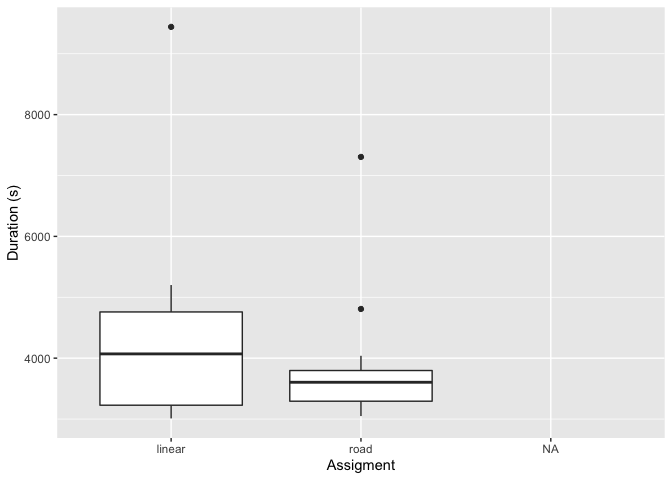
\includegraphics{cabify_challenge_files/figure-latex/unnamed-chunk-9-1.pdf}

Slightly shorter median duration is observed for the \emph{road}
assignment, but not significant.

Next, one could wonder whether these results are city-dependent. Bigger
and complex cities could be benefited by \emph{road} as traffic
assessments could help decide the best routes, while smaller cities
could not show the same benefits.

To test this, we repeated the analysis but controlling by city:

\begin{Shaded}
\begin{Highlighting}[]
\NormalTok{p3 }\OtherTok{\textless{}{-}} \FunctionTok{ggplot}\NormalTok{(}\FunctionTok{aes}\NormalTok{(}\AttributeTok{y =} \FunctionTok{as.numeric}\NormalTok{(duration), }\AttributeTok{x =} \FunctionTok{as.factor}\NormalTok{(city\_id), }
                 \AttributeTok{fill =} \FunctionTok{as.factor}\NormalTok{(trip\_id)), }\AttributeTok{data =}\NormalTok{ df\_sub) }\SpecialCharTok{+} \FunctionTok{geom\_boxplot}\NormalTok{() }
\NormalTok{p3 }\SpecialCharTok{+} \FunctionTok{xlab}\NormalTok{(}\StringTok{"City"}\NormalTok{) }\SpecialCharTok{+} \FunctionTok{ylab}\NormalTok{(}\StringTok{"Duration (s)"}\NormalTok{) }\SpecialCharTok{+} \FunctionTok{theme}\NormalTok{(}\AttributeTok{legend.title=}\FunctionTok{element\_blank}\NormalTok{()) }
\end{Highlighting}
\end{Shaded}

\begin{verbatim}
## Warning in FUN(X[[i]], ...): NAs introduced by coercion

## Warning in FUN(X[[i]], ...): NAs introduced by coercion
\end{verbatim}

\begin{verbatim}
## Warning: Removed 299 rows containing non-finite values (stat_boxplot).
\end{verbatim}

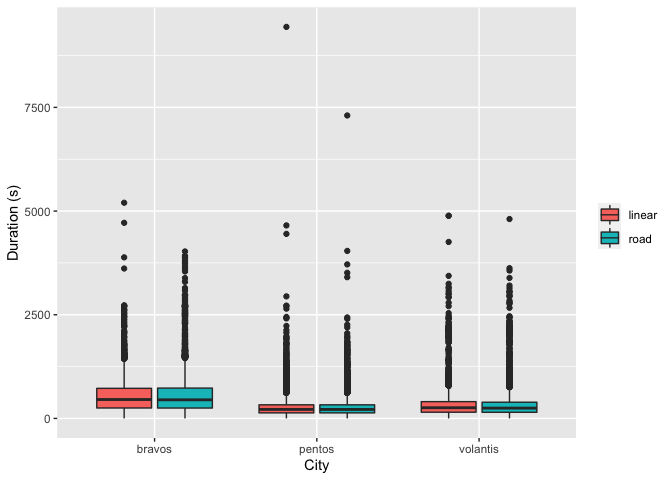
\includegraphics{cabify_challenge_files/figure-latex/unnamed-chunk-10-1.pdf}

Volantis seems to be benefited by the \emph{road} assignment, but a
formal test for the equality of the means must be performed to be able
to infer conclusions. The same methodology was used as in previous
sections. First, the normality of the distribution was checked. As the
distribution of the data was not normal, a Wilcoxon test was used.

\begin{Shaded}
\begin{Highlighting}[]
\NormalTok{df\_bravos }\OtherTok{\textless{}{-}}\NormalTok{ df\_sub[df\_sub}\SpecialCharTok{$}\NormalTok{city\_id}\SpecialCharTok{==}\StringTok{"bravos"}\NormalTok{,]}
\NormalTok{df\_pentos }\OtherTok{\textless{}{-}}\NormalTok{ df\_sub[df\_sub}\SpecialCharTok{$}\NormalTok{city\_id}\SpecialCharTok{==}\StringTok{"pentos"}\NormalTok{,]}
\NormalTok{df\_volantis }\OtherTok{\textless{}{-}}\NormalTok{ df\_sub[df\_sub}\SpecialCharTok{$}\NormalTok{city\_id}\SpecialCharTok{==}\StringTok{"volantis"}\NormalTok{,]}
\CommentTok{\# Normality test}
\FunctionTok{with}\NormalTok{(df\_bravos[}\FunctionTok{sample}\NormalTok{(}\DecValTok{1}\SpecialCharTok{:}\FunctionTok{nrow}\NormalTok{(df\_bravos),}\DecValTok{5000}\NormalTok{),], }
     \FunctionTok{shapiro.test}\NormalTok{(}\FunctionTok{as.numeric}\NormalTok{(duration[trip\_id }\SpecialCharTok{==} \StringTok{"linear"}\NormalTok{]))) }\CommentTok{\#p{-}value \textless{} 2.2e{-}16}
\end{Highlighting}
\end{Shaded}

\begin{verbatim}
## Warning in stopifnot(is.numeric(x)): NAs introduced by coercion
\end{verbatim}

\begin{Shaded}
\begin{Highlighting}[]
\FunctionTok{with}\NormalTok{(df\_pentos[}\FunctionTok{sample}\NormalTok{(}\DecValTok{1}\SpecialCharTok{:}\FunctionTok{nrow}\NormalTok{(df\_pentos),}\DecValTok{5000}\NormalTok{),], }
     \FunctionTok{shapiro.test}\NormalTok{(}\FunctionTok{as.numeric}\NormalTok{(duration[trip\_id }\SpecialCharTok{==} \StringTok{"linear"}\NormalTok{]))) }\CommentTok{\#p{-}value \textless{} 2.2e{-}16}
\end{Highlighting}
\end{Shaded}

\begin{verbatim}
## Warning in stopifnot(is.numeric(x)): NAs introduced by coercion
\end{verbatim}

\begin{Shaded}
\begin{Highlighting}[]
\FunctionTok{with}\NormalTok{(df\_volantis[}\FunctionTok{sample}\NormalTok{(}\DecValTok{1}\SpecialCharTok{:}\FunctionTok{nrow}\NormalTok{(df\_volantis),}\DecValTok{5000}\NormalTok{),], }
     \FunctionTok{shapiro.test}\NormalTok{(}\FunctionTok{as.numeric}\NormalTok{(duration[trip\_id }\SpecialCharTok{==} \StringTok{"linear"}\NormalTok{]))) }\CommentTok{\#p{-}value \textless{} 2.2e{-}16}
\end{Highlighting}
\end{Shaded}

\begin{verbatim}
## Warning in stopifnot(is.numeric(x)): NAs introduced by coercion
\end{verbatim}

\begin{Shaded}
\begin{Highlighting}[]
\CommentTok{\# Equality of means test}
\FunctionTok{wilcox.test}\NormalTok{(}\FunctionTok{as.numeric}\NormalTok{(df\_bravos}\SpecialCharTok{$}\NormalTok{duration[df\_bravos}\SpecialCharTok{$}\NormalTok{trip\_id}\SpecialCharTok{==}\StringTok{"road"}\NormalTok{]),}
            \FunctionTok{as.numeric}\NormalTok{(df\_bravos}\SpecialCharTok{$}\NormalTok{duration[df\_bravos}\SpecialCharTok{$}\NormalTok{trip\_id}\SpecialCharTok{==}\StringTok{"linear"}\NormalTok{]), }
            \AttributeTok{alternative =} \StringTok{"two.sided"}\NormalTok{)                        }\CommentTok{\#p{-}value = 0.5828}
\end{Highlighting}
\end{Shaded}

\begin{verbatim}
## Warning in wilcox.test(as.numeric(df_bravos$duration[df_bravos$trip_id == : NAs
## introduced by coercion
\end{verbatim}

\begin{verbatim}
## Warning in wilcox.test.default(as.numeric(df_bravos$duration[df_bravos$trip_id
## == : NAs introduced by coercion
\end{verbatim}

\begin{Shaded}
\begin{Highlighting}[]
\FunctionTok{wilcox.test}\NormalTok{(}\FunctionTok{as.numeric}\NormalTok{(df\_pentos}\SpecialCharTok{$}\NormalTok{duration[df\_pentos}\SpecialCharTok{$}\NormalTok{trip\_id}\SpecialCharTok{==}\StringTok{"road"}\NormalTok{]),}
            \FunctionTok{as.numeric}\NormalTok{(df\_pentos}\SpecialCharTok{$}\NormalTok{duration[df\_pentos}\SpecialCharTok{$}\NormalTok{trip\_id}\SpecialCharTok{==}\StringTok{"linear"}\NormalTok{]), }
            \AttributeTok{alternative =} \StringTok{"two.sided"}\NormalTok{)                        }\CommentTok{\#p{-}value = 0.9311}
\end{Highlighting}
\end{Shaded}

\begin{verbatim}
## Warning in wilcox.test(as.numeric(df_pentos$duration[df_pentos$trip_id == : NAs
## introduced by coercion
\end{verbatim}

\begin{verbatim}
## Warning in wilcox.test.default(as.numeric(df_pentos$duration[df_pentos$trip_id
## == : NAs introduced by coercion
\end{verbatim}

\begin{Shaded}
\begin{Highlighting}[]
\FunctionTok{wilcox.test}\NormalTok{(}\FunctionTok{as.numeric}\NormalTok{(df\_volantis}\SpecialCharTok{$}\NormalTok{duration[df\_volantis}\SpecialCharTok{$}\NormalTok{trip\_id}\SpecialCharTok{==}\StringTok{"road"}\NormalTok{]),}
            \FunctionTok{as.numeric}\NormalTok{(df\_volantis}\SpecialCharTok{$}\NormalTok{duration[df\_volantis}\SpecialCharTok{$}\NormalTok{trip\_id}\SpecialCharTok{==}\StringTok{"linear"}\NormalTok{]), }
            \AttributeTok{alternative =} \StringTok{"two.sided"}\NormalTok{)                        }\CommentTok{\#p{-}value = 0.3462}
\end{Highlighting}
\end{Shaded}

\begin{verbatim}
## Warning in wilcox.test(as.numeric(df_volantis$duration[df_volantis$trip_id == :
## NAs introduced by coercion
\end{verbatim}

\begin{verbatim}
## Warning in
## wilcox.test.default(as.numeric(df_volantis$duration[df_volantis$trip_id == : NAs
## introduced by coercion
\end{verbatim}

The W and p-values show that it cannot be concluded that the means are
different. The duration of the travel of each assignment is equal for
each city as well.

Finally, one could think there could exist differences between
\emph{road} and \emph{linear} for different times of the day. For
example, one could think than during peak hours (getting/going back from
work) the \emph{normal} assignment could mean faster trips due to the
capability of predicting traffic jams. To check this, a similar analysis
to previous parts was done. The duration data was grouped into 12
intervals, by dividing the started\_at values into 12 groups.

We create the one boxplot for each time interval (the whole time series
divided by 12):

\begin{Shaded}
\begin{Highlighting}[]
\CommentTok{\# Start\_time is broken into 12 intervals}
\NormalTok{df\_sub}\SpecialCharTok{$}\NormalTok{tinterv }\OtherTok{\textless{}{-}} \FunctionTok{as.numeric}\NormalTok{(}\FunctionTok{cut}\NormalTok{(df\_sub}\SpecialCharTok{$}\NormalTok{started\_at, }\AttributeTok{breaks =} \DecValTok{12}\NormalTok{))}
\CommentTok{\# Boxplots are plotted for each time interval}
\NormalTok{p4 }\OtherTok{\textless{}{-}} \FunctionTok{ggplot}\NormalTok{(}\FunctionTok{aes}\NormalTok{(}\AttributeTok{y =} \FunctionTok{as.numeric}\NormalTok{(duration), }\AttributeTok{x =} \FunctionTok{as.factor}\NormalTok{(tinterv), }\AttributeTok{fill =} 
                   \FunctionTok{as.factor}\NormalTok{(trip\_id)), }\AttributeTok{data =}\NormalTok{ df\_sub) }\SpecialCharTok{+} \FunctionTok{geom\_boxplot}\NormalTok{() }
\NormalTok{p4 }\SpecialCharTok{+} \FunctionTok{xlab}\NormalTok{(}\StringTok{"Day interval"}\NormalTok{) }\SpecialCharTok{+} \FunctionTok{ylab}\NormalTok{(}\StringTok{"Duration (s)"}\NormalTok{) }\SpecialCharTok{+} \FunctionTok{theme}\NormalTok{(}\AttributeTok{legend.title=}\FunctionTok{element\_blank}\NormalTok{()) }
\end{Highlighting}
\end{Shaded}

\begin{verbatim}
## Warning in FUN(X[[i]], ...): NAs introduced by coercion

## Warning in FUN(X[[i]], ...): NAs introduced by coercion
\end{verbatim}

\begin{verbatim}
## Warning: Removed 299 rows containing non-finite values (stat_boxplot).
\end{verbatim}

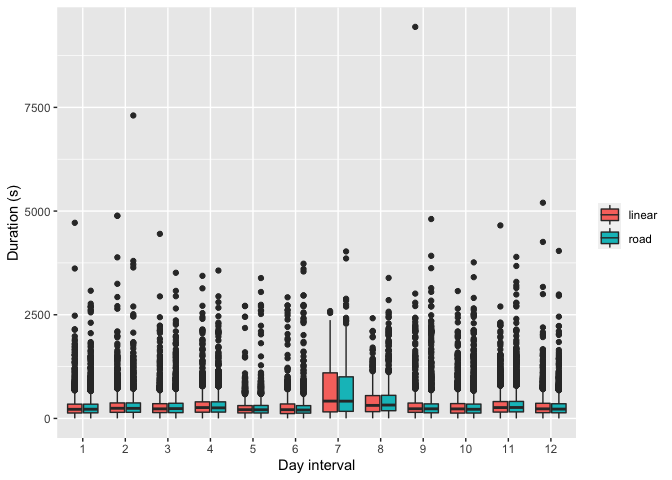
\includegraphics{cabify_challenge_files/figure-latex/unnamed-chunk-12-1.pdf}

We can see that the differences between \emph{road} and \emph{linear}
are minimal for most of the time intervals. The time interval with a
higher difference was the interval 7, but in this case the \emph{linear}
durations were shorter than those of the \emph{road} assignment.

\textbf{1. Should the company move towards road distance? What's the max
price it would make sense to pay per query? (make all the assumptions
you need, and make them explicit)}

The analysis showed that the trips of the vehicles that were picking up
customers did not differ in duration from the group that used the
\emph{linear} assignment than the group that used \emph{road}
assignment. We can conclude from this that the company should not move
towards the road distance. The \emph{road} service comes with certain
cost and increases the complexity of the system, potentially decreasing
its reliability. After observing that the use of this service does not
translate into faster trips to picking up costumers, it is safe to say
that it should not be used.

A maximum price for each query of the \emph{road} service was not
calculated as any value bigger than zero would not be worth it, because
the analysis showed that the difference in duration from the two systems
can be due just to randomness and not an improvement of the speed due to
the \emph{road} service.

A different question would be if the \emph{road} system improves the gas
consumption due to avoiding less energy-efficient routes. For example,
\emph{road} takes the same time to arrive to destination, but through a
route free of traffic lights were the gas consumption is reduced. In
this case, \emph{road} system would have benefits. But because the
question was related to the benefits for the time-reducement to pick up
to the costumer, the answer is that the company should not move towards
road distance.

\textbf{2. How would you improve the experimental design? Would you
collect any additional data?}

There are a few aspects that could be improved from the experimental
design. First, the experiment has been done in three cities with very
similar duration times. This means that the size of the city, or the
density of drivers is similar between them (although the time duration
for Bravos was significantly higher than the other two). To obtain less
biased results, a wide range of cities presenting a range of durations
(which would mean a range of city size or drivers density) would be
needed. This could show, for example, that for cities with lower density
of drivers, the \emph{road} system might have some advantage.

An interesting additional data to collect during the experiment would
have been the driver's coordinates (initial and final). Making the
problem spatially explicit could have provided more insides of the
advantages/disadvantages of each system. For example, adding coordinates
would have allowed to make a study based in regions. In more populated
areas, or with more costumers, or with higher traffic densities,
differences between \emph{road} and \emph{linear} systems could have
arised.

\end{document}
